\documentclass{standalone}
\usepackage{tikz}
\usetikzlibrary{matrix,arrows,decorations.pathmorphing,decorations.pathreplacing,calc,positioning}
\usepackage{xcolor}
% all other packages and stuff you need for the picture
\newcommand{\myunit}{0.65 cm}
\newcommand{\myraise}{3pt}
\tikzset{
    lpltsty/.style={decorate, decoration = {brace,mirror,raise=3pt,amplitude=5pt}},
    namesty/.style={pos=0.5,below=7pt},
    scalarsty/.style={draw,fill=white,rectangle,minimum size=\myunit,anchor=center},
    indexsty/.style={fill,fill=white,rectangle,minimum width=\myunit,anchor=center},
    touchsty/.style={fill,fill=red,rectangle,minimum size=\myunit},
    ycsty/.style={fill,fill=yellow,rectangle,minimum size=\myunit},
    fullsty/.style={draw,fill=zerogray,rectangle,minimum size=\myunit},
    brcsty/.style={fill,fill=brown,rectangle,minimum size=\myunit},
    blcsty/.style={fill,fill=cyan!20,rectangle,minimum size=\myunit},
    becsty/.style={fill,fill=beige,rectangle,minimum size=\myunit},
    ocsty/.style={fill,fill=orange,rectangle,minimum size=\myunit},
    whclsty/.style={fill,fill=white,rectangle,minimum size=\myunit},
    zcsty/.style={fill,fill=white,rectangle,minimum size=\myunit,text=zerogray},
    nzsty/.style={fill,fill=black,rectangle,minimum size=\myunit,text=white},
    rcsty/.style={fill,fill=purple,rectangle,minimum size=\myunit},
    pcsty/.style={fill,fill=pink,rectangle,minimum size=\myunit},
    lcsty/.style={fill,fill=blue,rectangle,minimum size=\myunit},
    bcsty/.style={fill,fill=black,rectangle,minimum size=\myunit, text=white},
    hlsty/.style={draw=red},
}


\colorlet{zerogray}{gray!25}
\colorlet{beige}{brown!70}

\newcommand{\ylcl}{|[ycsty]|1}
\newcommand{\recl}{|[rcsty]|2}
\newcommand{\picl}{|[pcsty]|3}
\newcommand{\blcl}{|[blcsty]|1}
\newcommand{\brcl}{|[brcsty]|2}
\newcommand{\becl}{|[becsty]|3}
\newcommand{\orcl}{|[ocsty]|4}
\newcommand{\bkcl}{|[bcsty]|5}
\newcommand{\whcl}{|[whclsty]|0}
\newcommand{\zecl}{|[zcsty]|0}

\newcommand{\formatscale}{0.5}
\newcommand{\matrixscale}{0.69}
\begin{document}
\resizebox{\linewidth}{!}{%
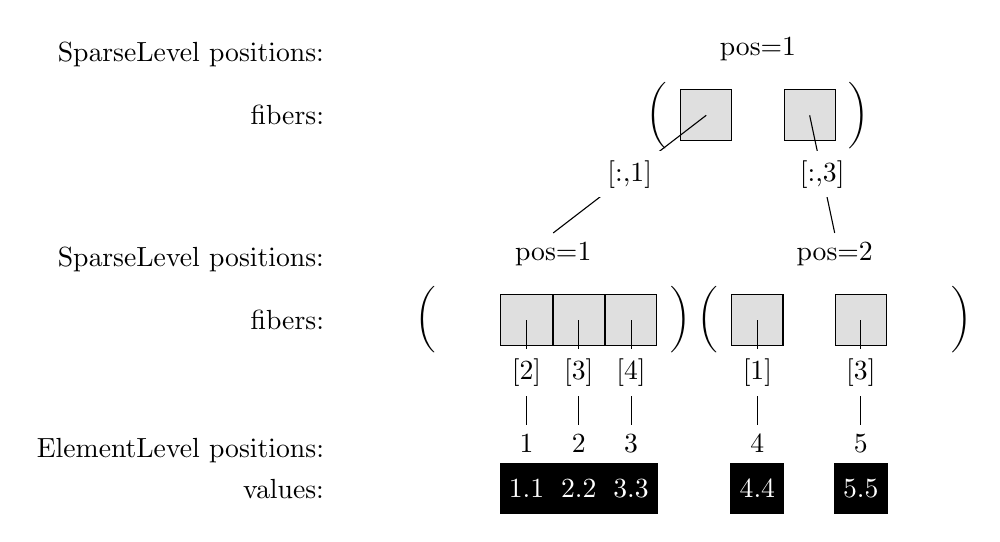
\begin{tikzpicture}[>=latex]

\node (Ad2p1l) [anchor=north] at (6.75*\myunit, 0*\myunit) {pos=1};
\matrix (Ad2p1) [matrix of math nodes,
    nodes = {whclsty},
    left delimiter  = (,
    right delimiter = ),
    ampersand replacement=\&,
    anchor=north] at (6.75*\myunit, -1*\myunit)
{
|[fullsty]|\&|[zcsty]|\&|[fullsty]|\\
};
\node (Ad1p1l) [anchor=north] at (2.75*\myunit, -4*\myunit) {pos=1};
\matrix (Ad1p1) [matrix of math nodes,
    nodes = {whclsty},
    left delimiter  = (,
    right delimiter = ),
    ampersand replacement=\&,
    anchor=north] at (2.75*\myunit, -5*\myunit)
{
|[zcsty]|\&|[fullsty]|\&|[fullsty]|\&|[fullsty]|\\
};
\node (Ad0p1l) [below=of Ad1p1-1-2] {\\1};
\node (Ad0p1) [below=0 of Ad0p1l.south, nzsty] {1.1};
\draw (Ad1p1-1-2.center) -- (Ad0p1l.north) node [midway, fill=white] {[2]};
\node (Ad0p2l) [below=of Ad1p1-1-3] {\\2};
\node (Ad0p2) [below=0 of Ad0p2l.south, nzsty] {2.2};
\draw (Ad1p1-1-3.center) -- (Ad0p2l.north) node [midway, fill=white] {[3]};
\node (Ad0p3l) [below=of Ad1p1-1-4] {\\3};
\node (Ad0p3) [below=0 of Ad0p3l.south, nzsty] {3.3};
\draw (Ad1p1-1-4.center) -- (Ad0p3l.north) node [midway, fill=white] {[4]};
\draw (Ad2p1-1-1.center) -- (Ad1p1l.north) node [midway, fill=white] {[:,1]};
\node (Ad1p2l) [anchor=north] at (8.25*\myunit, -4*\myunit) {pos=2};
\matrix (Ad1p2) [matrix of math nodes,
    nodes = {whclsty},
    left delimiter  = (,
    right delimiter = ),
    ampersand replacement=\&,
    anchor=north] at (8.25*\myunit, -5*\myunit)
{
|[fullsty]|\&|[zcsty]|\&|[fullsty]|\&|[zcsty]|\\
};
\node (Ad0p4l) [below=of Ad1p2-1-1] {\\4};
\node (Ad0p4) [below=0 of Ad0p4l.south, nzsty] {4.4};
\draw (Ad1p2-1-1.center) -- (Ad0p4l.north) node [midway, fill=white] {[1]};
\node (Ad0p5l) [below=of Ad1p2-1-3] {\\5};
\node (Ad0p5) [below=0 of Ad0p5l.south, nzsty] {5.5};
\draw (Ad1p2-1-3.center) -- (Ad0p5l.north) node [midway, fill=white] {[3]};
\draw (Ad2p1-1-3.center) -- (Ad1p2l.north) node [midway, fill=white] {[:,3]};
\draw [whclsty, anchor=north east] let \p1 = (Ad2p1-1-1.north) in (-1, \y1) node {fibers:};
\draw [whclsty, anchor=north east] let \p1 = (Ad2p1l.north) in (-1, \y1) node {SparseLevel positions:};

\draw [whclsty, anchor=north east] let \p1 = (Ad1p1-1-1.north) in (-1, \y1) node {fibers:};
\draw [whclsty, anchor=north east] let \p1 = (Ad1p1l.north) in (-1, \y1) node {SparseLevel positions:};

\draw [whclsty, anchor=north east] let \p1 = (Ad0p1.north) in (-1, \y1) node {values:};
\draw [whclsty, anchor=north east] let \p1 = (Ad0p1l.north) in (-1, \y1) node {ElementLevel positions:};

\end{tikzpicture}%
}
\end{document}

